
\documentclass[a4paper,kul]{kulakarticle} %options: kul or kulak (default)

\usepackage[utf8]{inputenc}
\usepackage[dutch]{babel}
\usepackage{graphicx}
\usepackage{hyperref}
\usepackage{caption}
\usepackage{subcaption}

\date{31/05/2019}
\address{
  Faculteit Industriële Ingenieurswetenschappen \\
  Projectlab bachelor elektronica-ICT \\
  J. Lannoo, L. Espeel}
\title{Verslag E-ink room reservation display}
\author{Baptiste Pattyn\and Michel Dequick \and Stijn Declerck \and Ine Vanderhaeghe}


\begin{document}

\maketitle

\begin{center}
	\centering
	\vspace*{\fill}
	\huge
	\textbf{E-ink room reservation display}
	\vspace*{\fill}
\end{center}

\newpage

\section{Inhoud}

\tableofcontents

\newpage

\section{Probleemstelling}

We willen een display maken voor klaslokalen die dynamisch kan veranderen per uur. 

Op het scherm moeten verschillende zaken komen: het nummer van het klaslokaal, de datum, op welke uren het lokaal bezet is op die dag, welk vak op dit moment gegeven wordt en de docent die dit vak geeft.
\newline

Er zijn verschillende dingen waar we rekening mee moeten houden om dit te realiseren:

We moeten een E-ink display implementeren. Hierbij moeten we bekijken als hier burn-in of ghosting kan optreden. Ook moeten we rekening houden met de grootte van de memory in de display.

Er moet een databank opgezet worden waar alle data van de lokalen in opgeslagen is. Deze databank moet bereikbaar zijn via wifi.

Er moet een connectie gemaakt worden via een wifi module van de databank naar de display.
\newline

We gebruiken hiervoor een E-ink display omdat dit het meest energiezuinig is. Dit komt omdat de display enkel voeding nodig heeft om het scherm te veranderen. We moeten het scherm maar om het uur aanpassen, dus alle tijd daartussen heeft een E-ink display geen voeding nodig.
Een ander voordeel van een E-ink display is dat het geen licht uitzendt, maar het reflecteert licht zoals een blad papier. Hierdoor is het gemakkelijker leesbaar, ook als er in de omgeving veel licht is. 
\newline

De eenvoudigste E-ink display is de "two pigment ink system". Dit bestaat uit kleine gebieden die dipolen zijn (deze worden gebruikt als de pixels van de afbeelding). De positieve kant van de gebieden bestaat uit wit pigment, de negatieve kant is zwart pigment. Deze gebieden bevinden zich in een bubbel van olie zodat ze gemakkelijk kunnen omdraaien, en zitten tussen transparante elektrode lagen. Wanneer nu op die elektrode lagen een spanning wordt gezet, kan bepaald worden welke delen van het scherm zwart zijn, en welke wit. Op die manier kan een zwart-wit afbeelding op de display geprogrammeerd worden. (zie afbeelding \ref{fig:2psystem} ).

\begin{figure}[h]
	\centering
	\begin{subfigure}{.5\textwidth}
		\centering
		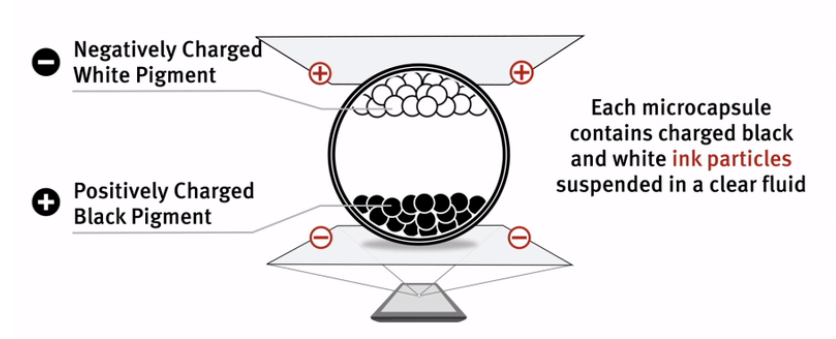
\includegraphics[width=0.95\textwidth]{Two_pigment_ink_system1}
		\label{fig:sub2psystem}
	\end{subfigure}%
	\begin{subfigure}{.5\textwidth}
		\centering
		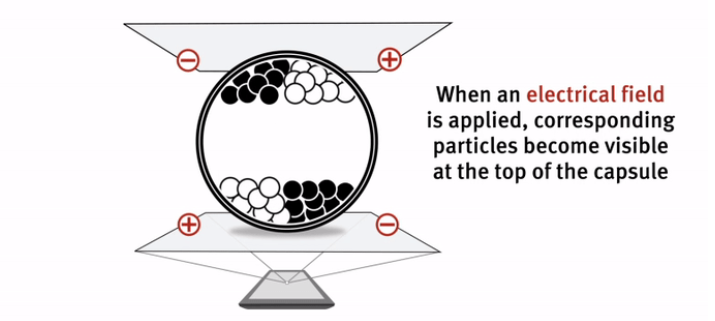
\includegraphics[width=0.95\textwidth]{Two_pigment_ink_system2}
		\label{fig:sub2psystem2}
	\end{subfigure}
	\caption{two pigment ink system}
	\label{fig:2psystem}
\end{figure}

Er bestaat ook een "Three pigment ink system". Dit werkt op ongeveer dezelfde manier als two pigment ink system (zie afbeelding \ref{fig:3psystem} ). Hier is het witte pigment negatief geladen en het rode pigment is positief geladen. Om het zwarte pigment aan de oppervlakte te brengen, moet er een gesplitste lading aangebracht worden.

\begin{figure}[h]
	\centering
	\begin{subfigure}{.5\textwidth}
		\centering
		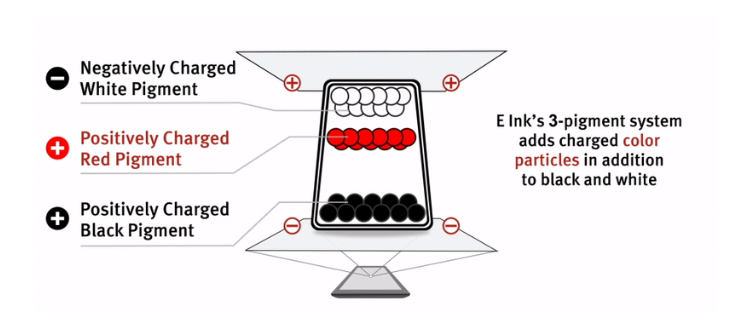
\includegraphics[width=0.95\textwidth]{three_pigment_ink_system1}
		\label{fig:sub3psystem}
	\end{subfigure}%
	\begin{subfigure}{.5\textwidth}
		\centering
		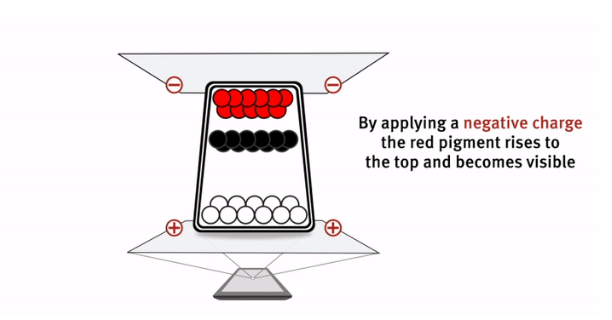
\includegraphics[width=0.95\textwidth]{three_pigment_ink_system2}
		\label{fig:sub3psystem2}
	\end{subfigure}
	\caption{three pigment ink system}
	\label{fig:3psystem}
\end{figure}

De E-ink display die wij gaan gebruiken, gebruikt het three pigment ink system. Op deze manier kunnen we op een overzichtelijke manier op een tijdslijn aanduiden op welke uren het lokaal bezet is.
\newline

Daarnaast bestaat er ook een "Advanced color ePaper". Hierbij kunnen nog meer kleuren op het scherm afgebeeld worden. (zie afbeelding \ref{fig:ACeP} ). Dit gebruiken wij niet in dit project. Dit systeem gebruikt 4 kleuren: cyaan, magenta, geel en wit.  \newline

\begin{figure}[h]
	\centering
	\begin{subfigure}{.5\textwidth}
		\centering
		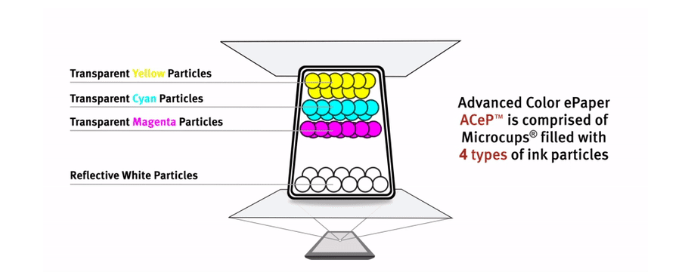
\includegraphics[width=0.95\textwidth]{ACeP1}
		\label{fig:subACeP}
	\end{subfigure}%
	\begin{subfigure}{.5\textwidth}
		\centering
		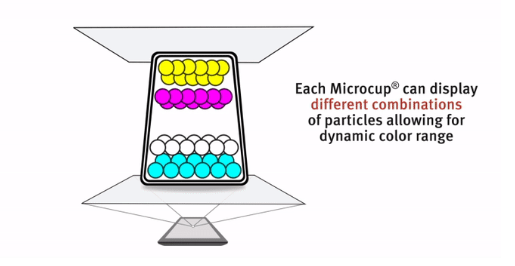
\includegraphics[width=0.95\textwidth]{ACeP2}
		\label{fig:subACeP2}
	\end{subfigure}
	\caption{Advanced color ePaper}
	\label{fig:ACeP}
\end{figure}

bron figuren: \cite{E-ink}.

bron werking ACeP: \cite{ACeP}.
\newline
\newline
Dit is het materiaal dat we gebruikt hebben:
\newline
Mbed FRDM-K64F

met application shield en click shield
\newline
ESP-WROOM-02 click met ESP8266EX wifi bord

Datasheet ESP-WROOM-02: \cite{ESP-WROOM-02}

Datasheet ESP8266EX: \cite{ESP8266EX}
\newline
Eink click, small and big display

\newpage

\section{Aanpak}

Eerst hebben we alle deelopdrachten op een rijtje gezet en een planning gemaakt. Daarbij hebben we ook een taakverdeling gemaakt. 
\newline
\newline
Dit zijn de grootste taken:
\newline
\newline
Een library maken voor de display – Michel
\newline
Eerst moesten we bekijken hoe we een afbeelding op de display konden krijgen. Op het internet vonden we een voorbeeld van een E-ink display die gemaakt was met een Arduino. Wij maken gebruik van een mbed, dus we hebben de code moeten aanpassen. 
Als eerste hebben we geprobeerd om een afbeelding op de display te zetten en om een afbeelding die er op staat te kunnen wissen.
Daarna hebben we een ontwerp gemaakt van wat we allemaal op het scherm wilden zetten en waar. We hebben dan ook geprobeerd om dit op de display te krijgen.
\newline
\newline
Een database opstellen met een wifi access point – Baptiste
\newline
We hebben een database opgesteld op een Raspberry Pi. Daar hebben we ook een wifi access point op geïmplementeerd zodat de display met de databank kan communiceren.
Eens de databank opgevuld was konden we testen als we de data konden in een tabel zetten per lokaal.
\newline
\newline
Wifi connectiviteit en JSON parser maken – Stijn
\newline
Het is belangrijk om via wifi te kunnen communiceren tussen de E-ink display en de databank. Hiervoor moesten we onderzoeken hoe een HTTP GET request werkt en het hoe we het zelf konden implementeren in onze toepassing.
\newline
We moeten ook een manier hebben om de data te versturen. Hiervoor moest een JSON parser gemaakt worden.
\newline
\newline
Er waren ook enkele kleinere taken:
\newline
\newline
De databank invullen – Ine
\newline
De databank moest opgevuld worden met fictieve data over de lokaalbezetting zodat we een proof of concept konden maken om voor te stellen op de presentatie van ons project.
\newline
\newline
Het verslag en de powerpointpresentatie opstarten – Ine 
\newline
Om het verslag te maken heeft iedereen het deel ingevuld waar hij zelf meest aan gewerkt heeft aangevuld. 

\newpage

\section{Implementatie}
\subsection{Database en Wifi Access Point}
Voor het opslaan van de gegevens is er een database opgezet op een Raspberry Pi model B+ door gebruik te maken van phpMyAdmin. Hier draait een SQL server op waarin alle gegevens voor de komende events van verschillende lokalen kunnen opgeslagen worden. Verder zijn alle gegevens van de courses er ook opgeslagen en de algemene info van de rooms. Om ervoor te zorgen dat onze MBED toegang kan krijgen tot deze database hebben we een Wifi Access Point (WAP) op de Raspberry Pi gezet, waarmee de MBED zich kan verbinden via een ESP8266 Wifi chip. Het opvragen van de gegevens door de mbed gebeurt via een GET request op de HTTP poort van de Raspberry Pi (poort 80).
 
\subsubsection{Database}
Deze database genaamd roomdb bestaat uit 3 verschillende tables: courses, events en rooms. De structuur van de database en de relaties tussen de verschillende tables staat afgebeeld in figuur \ref{fig:dbstruct}. Op de Raspberry Pi staan verschillende PHP files die ervoor zorgen dat de webserver kan verbinden met de database. Een belangrijke file hierbij is dbConnect.php (zie figuur \ref{fig:dbconnect}), in deze file staan de gegevens die nodig zijn om te kunnen verbinden met de database. In deze  file declareren we verschillende variabelen: \verb|$host|, \verb|$user|, \verb|$password|en \verb|$databse|. Deze worden dan gebruikt in een \verb|mysqli_connect()| commando om een verbinding op te zetten met de databse. Hierna wordt er nog een controle gedaan om te kijken of de verbinding tot stand is gekomen, indien dit niet het geval is dan verkrijgen we een error. Deze code is enkel bedoeld voor tijdens het opzetten van de webserver en de database en dient verwijderd te worden indien de code definitief in gebruik wordt genomen. Als \verb|$host| kiezen we het local host adres 127.0.0.1 omdat de database zich op de Raspberry Pi zelf bevindt. De \verb|$user| en het \verb|$password| zijn specifiek voor elke database en hangen af van welke user je ingesteld hebt op je SQL server. 
\begin{figure}[h]
	\begin{verbatim}
	<?php
	$host = "127.0.0.1";
	$user = "root";
	$password = "password" ;
	$database = "roomdb";
	$conn = mysqli_connect($host, $user, $password, $database);
	// delete when ready to launch
	if(!$conn){
	die("Connection failed: " . $conn ->connect_error);
	}
	?>
	\end{verbatim}
	\caption{dbConnect.php}
	\label{fig:dbconnect}
\end{figure}
\begin{figure}[h]
	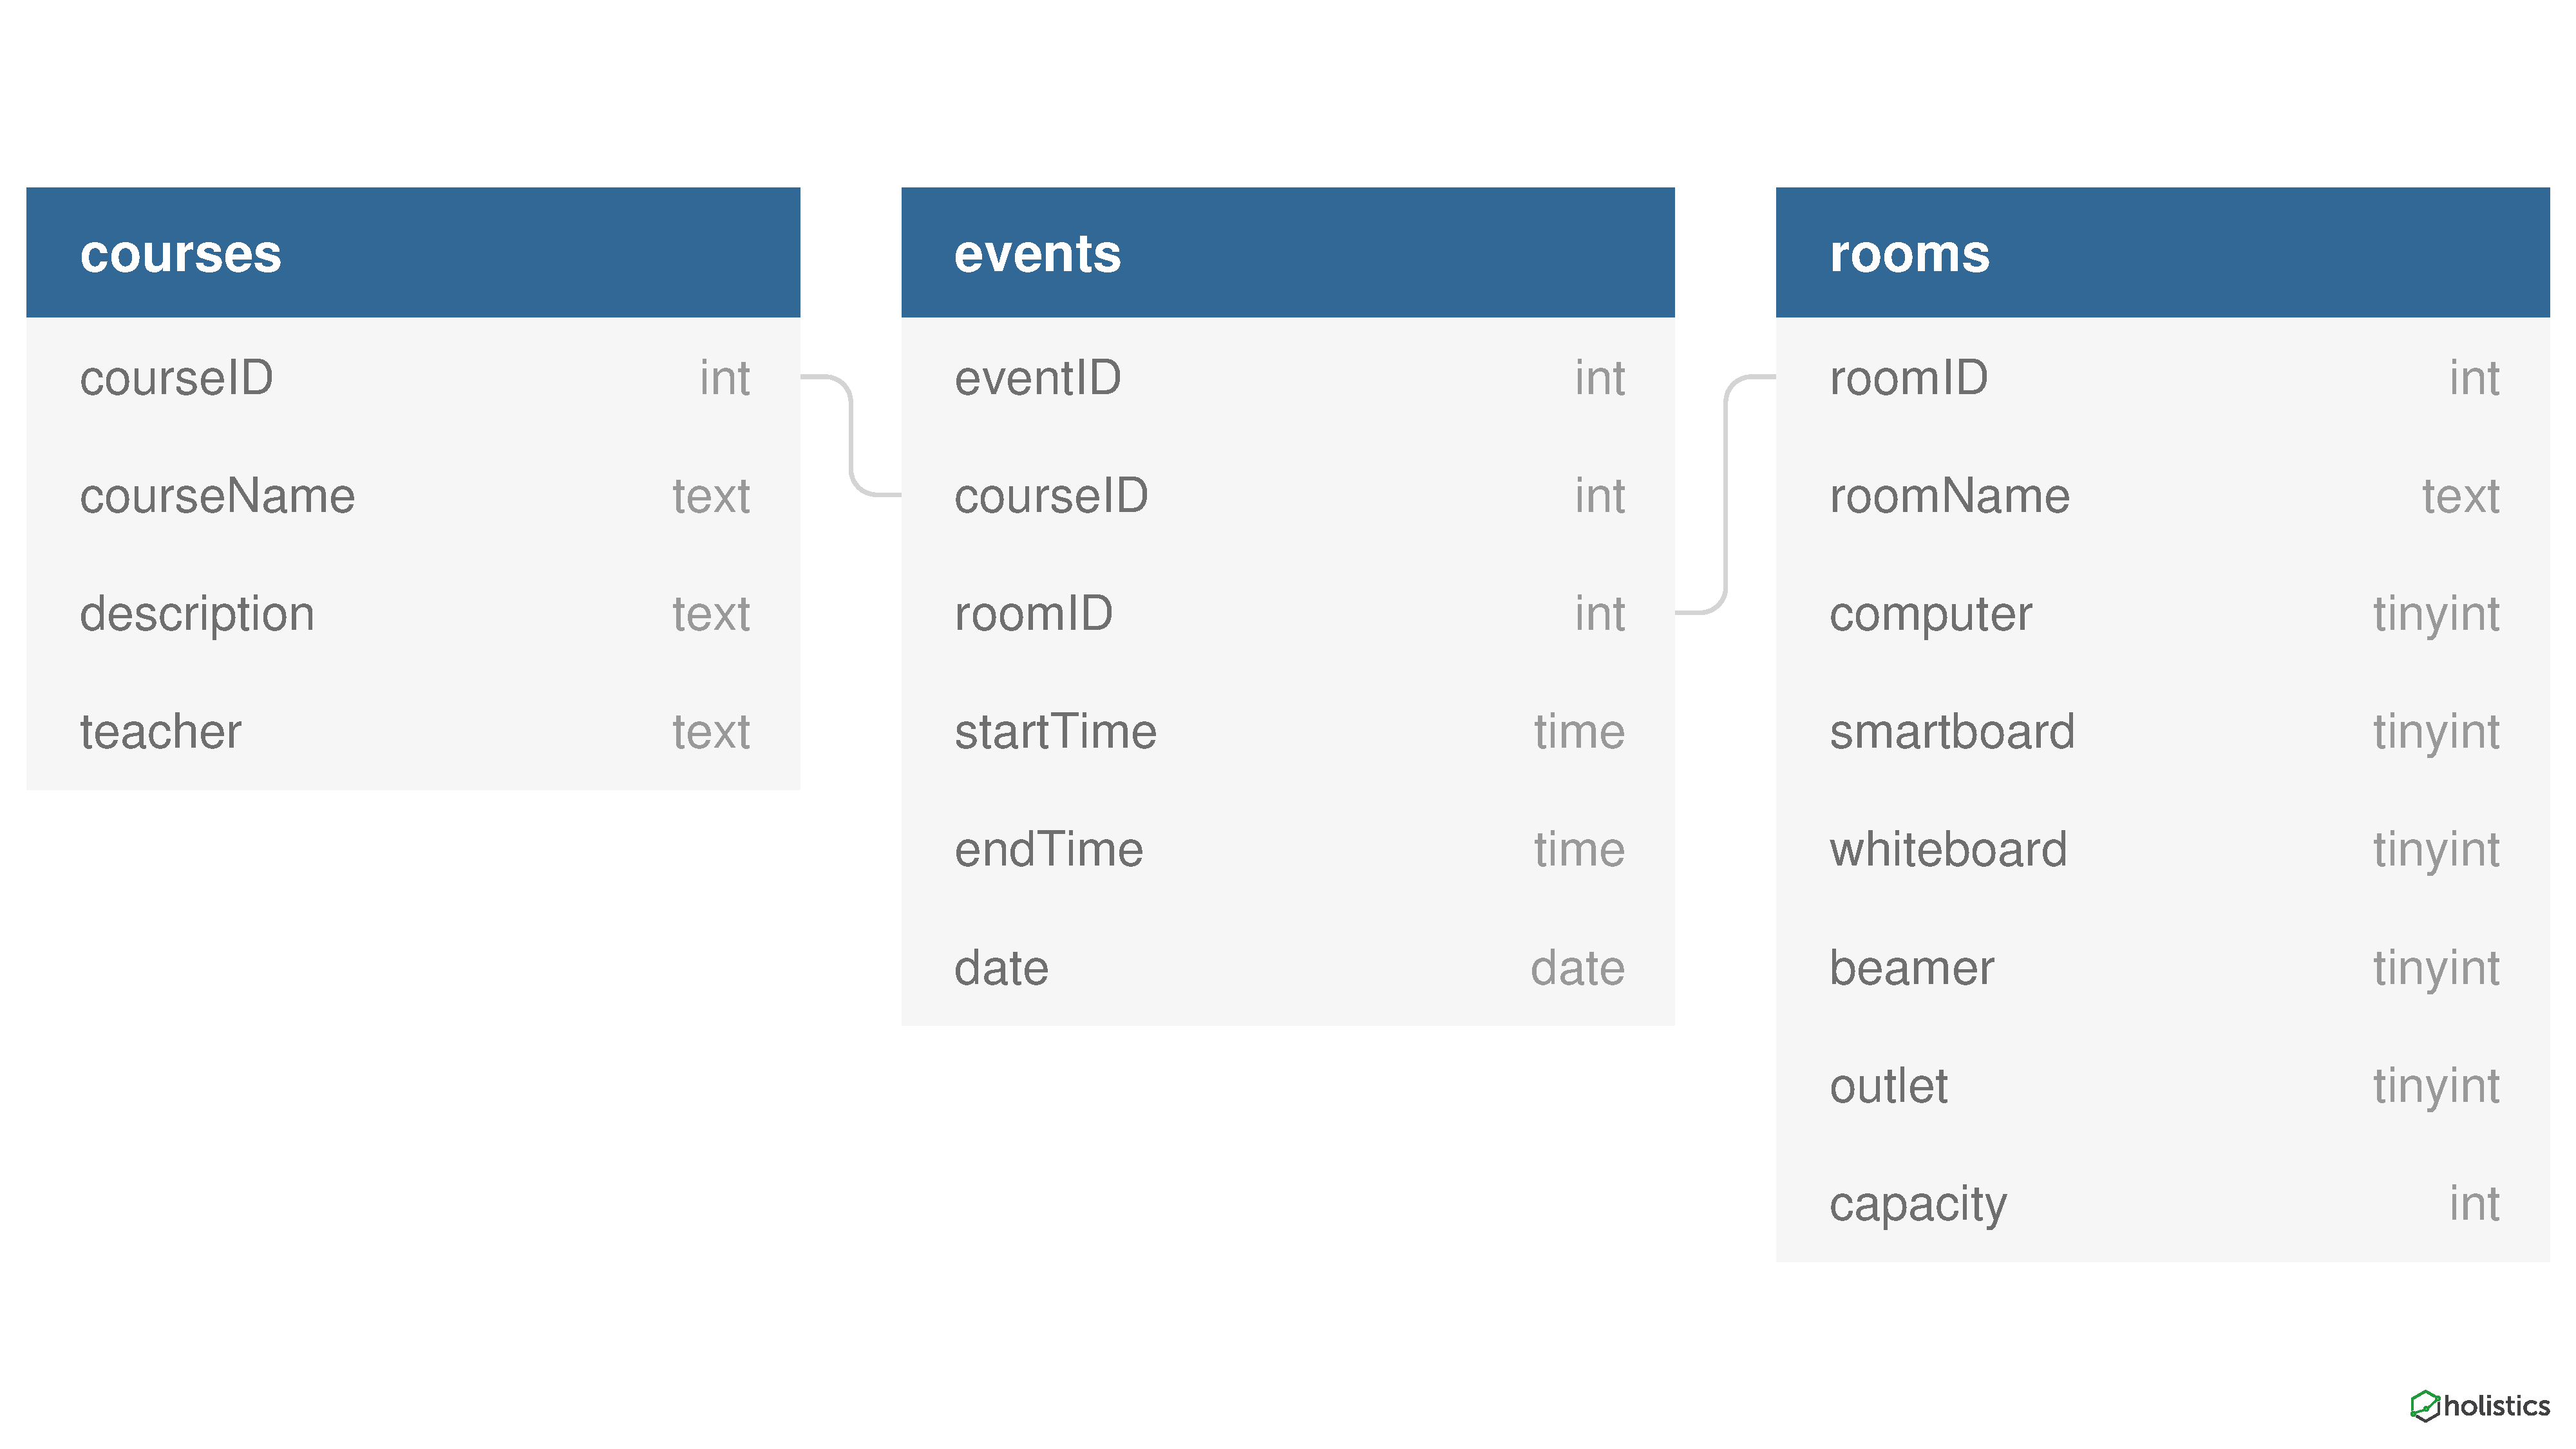
\includegraphics[width=0.9\textwidth]{dbstruct}
	\caption{Database structuur}
	\label{fig:dbstruct}
\end{figure}
\subsubsection{Wifi Access Point op Raspberry Pi}
Voor het opzetten van de WAP op de Raspberry Pi hebben we een online step-by-step guide gevolgd \cite{RaspberryPiWAP}. De belangrijkste services die we hiervoor installeren op de Raspberry Pi zijn \verb|hostapd| en \verb|dnsmasq|.
\paragraph{DNSmasq} \mbox{}\\ 
Deze service is in principe gewoon een DHCP (Dynamic Host Configuration Protocol) server. Deze zal ervoor zorgen dat we dynamisch IP adressen kunnen toekennen op ons netwerk zonder dat we alle apparaten manueel moeten verbinden. In de config file van dnsmasq (die zich onder het volgende path bevindt \verb|/etc/dnsmasq.conf|) kennen we een range aan van IP adressen die onze Wifi kan gebruiken om toe te kennen aan apparaten. Verder bepalen we ook hoelang deze IP adressen kunnen gebruikt worden door de apparaten die zich verbinden met het Wifi netwerk. De config file ziet er dan als volgt uit \ref{fig:dnsmasq} .
\begin{figure}[!h]
	\begin{verbatim}
	interface=wlan0
	dhcp-range=192.168.0.11,192.168.0.30,255.255.255.0,24h
	\end{verbatim}
	\caption{dnsmasq.conf}
	\label{fig:dnsmasq}
\end{figure}
\paragraph{Hostapd} \mbox{}\\
Deze service zorgt ervoor dat er een WAP wordt opgezet. In de config file van hostapd (die zich onder het volgende path bevindt \verb|/etc/hostapd/hostapd.conf|) stel je het SSID en het wachtwoord in van je WAP. Verder stel je hier ook een bridge in tussen je ethernet verbinding en je wlan0 van je Raspberry Pi. Dit zorgt ervoor dat je zowel via ethernet als via de WAP toegang kan krijgen tot je webserver. In deze file zorgen we ervoor dat we steeds op channel 7 zullen zitten van van de Wifi. We stellen ook de Wifi Protected Acces (WPA) versie in en bepalen welke vorm van management we zullen gebruiken voor het WPA wachtwoord. Voor deze opdracht gebruiken we WPA-PSK wat staat voor Pre-Shared Key. Een wachtwoord bestaat uit minimaal 8 en maximaal 63 tekens. De config file ziet er dan als volgt uit \ref{fig:hostapd} .
\begin{figure}[!h]
	\begin{verbatim}
	interface=wlan0
	driver=nl80211
	bridge=br0
	hw_mode=g
	channel=7
	wmm_enabled=0
	macaddr_acl=0
	auth_algs=1
	ignore_broadcast_ssid=0
	wpa=2
	wpa_key_mgmt=WPA-PSK
	wpa_pairwise=TKIP
	wpa_pairwise=CCMP
	ssid=teamzoepertoff
	wpa_passphrase=stijnkanniks
	\end{verbatim}
	\caption{hostapd.conf}
	\label{fig:hostapd}
\end{figure}
\newpage
\subsubsection{Webserver en GET request}
De webserver die we op onze Raspberry Pi draaien is een apache 2.4 server die de mogelijkheid heeft om samen te werken met onze SQL database. Voor onze applicatie hebben we slechts vier van de zes aanwezige files nodig: 
\begin{itemize}
	\item \verb|dbConnect.php|
	\item \verb|event.php|
	\item \verb|room.php|
	\item \verb|roominfo.php|
\end{itemize}
De overige twee files (\verb|index.php| en \verb|showTable.php|) zijn er enkel indien we via een webbrowser toegang willen krijgen tot de lokaalbezetting. Wanneer we een GET request sturen vanuit onze MBED dan slaan we de \verb|index.php| file over. Een GET request ziet er als volgt uit: \\ \verb|http://ip-address/E-ink-room/roominfo.php?roomName=02.85|. \\ We gaan dus rechtstreeks naar \verb|roominfo.php| en geven als variabele het nummer mee van het lokaal waarvan we de info willen verkrijgen.  De inhoud van \verb|dbConnect.php| hebben we hierboven al besproken, dus zullen we er hier niet meer verder op ingaan. \verb|event.php| en \verb|room.php|, zijn hele kleine files die beide \'{e}\'{e}n enkele klasse bevatten. De UML diagramma's voor deze klassen staan in figuur \ref{fig:uml}.
\begin{figure}[h]
	\centering
	\begin{subfigure}{0.45\textwidth}
		\centering
		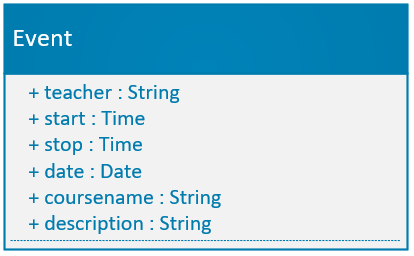
\includegraphics[width=0.95\textwidth]{EventUML.png}
	\end{subfigure}
	\begin{subfigure}{0.45\textwidth}
		\centering
		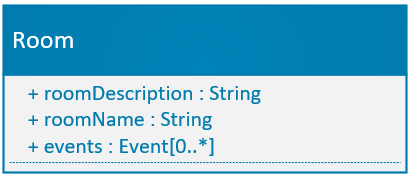
\includegraphics[width=0.95\textwidth]{RoomUML.png}
	\end{subfigure}
	\caption{UML diagram}
	\label{fig:uml}
\end{figure} \\
De laatste en tevens ook grootste file is \verb|roominfo.php|. Hierin worden de klassen die in de vorige files gedefinieerd werden gebruikt. Bij onze GET-request geven we een variabele mee die \verb|roomName| genaamd is. Deze slaan we dan op in een variabele die we \verb|$roomName| gaan noemen. Wegens veiligheidsredenen gaan we eerst de door de gebruiker meegegeven variabele sanitizen, dit zorgt ervoor dat er geen SQL code kan geïnjecteerd worden die er eventueel voor kan zorgen dat onze database aangepast wordt zonder dat wij dit willen. De methode die we hiervoor gebruiken is \verb|mysqli_real_escape_string(string $escapestr)|.

De variabele \verb|$roomName| kunnen we nu gebruiken om een query uit te voeren naar onze database om zo het \verb|roomID| en de \verb|roomDescription| te kunnen verkrijgen van het opgevraagde lokaal. Het opvragen van deze gegevens gebeurt volgens de code in figuur \ref{fig:roomsql}. Eerst wordt een statement aangemaakt via de \verb|prepare()| methode. Hierin zetten we de SQL code met de parameters die we willen selecteren en de voorwaarde die aangeeft welke entries van de database mogen opgehaald worden. De waarde van de variabele waarop geselecteerd wordt kennen we later toe met de \verb|bind_param()| methode. De eerste parameter geeft aan dat we selecteren op een variabele van het type String en de tweede parameter is de variabele zelf. Na de \verb|execute()| methode gebruiken we de \verb|bind_result()| methode om de variabelen van de opgehaalde database entry toe te kennen aan de correcte variabelen zodat we ze later kunnen gebruiken.  Het roomID hebben we nodig omdat we dan in onze event table kunnen zoeken naar alle geplande events die het opgegeven roomID bevatten.

\begin{figure}
	\begin{verbatim}
		$roomName = mysqli_real_escape_string($conn, $_GET['roomName']);
		$stmt = $conn->prepare("SELECT roomID, roomDescription FROM rooms WHERE roomName=?");
		$stmt->bind_param("s", $roomName);
		$stmt->execute();
		$stmt->bind_result($roomID, $roomDescription);
	\end{verbatim}
	\caption{Info over lokaal ophalen uit database}
	\label{fig:roomsql}
\end{figure}
\newpage
Na het ophalen van het roomID voeren we een SQL query uit om alle entries uit de events table te halen die doorgaan in het door ons opgevraagde lokaal. De resultaten van deze queries steken we dan in arrays, in de volgorde zoals ze uit de table gekomen zijn. Zo kunnen we gemakkelijk de verschillende variabelen opvragen door de indexen te gebruiken van de arrays. Alle elementen van een bepaald event bevinden zich namelijk op de plaats in de array met dezelfde index.De laatste stap is om via de courseID's de courseNames op te gaan vragen in de courses table en dan hebben we alle nodige info beschikbaar om terug te sturen naar de MBED.


\newpage

\section{Resultaten}

We kunnen uit de databank info van lokaal 02.85 filteren en in een tabel zetten. Zie figuur \ref{fig:vboutput}.

\begin{figure}[h]
	\centering
	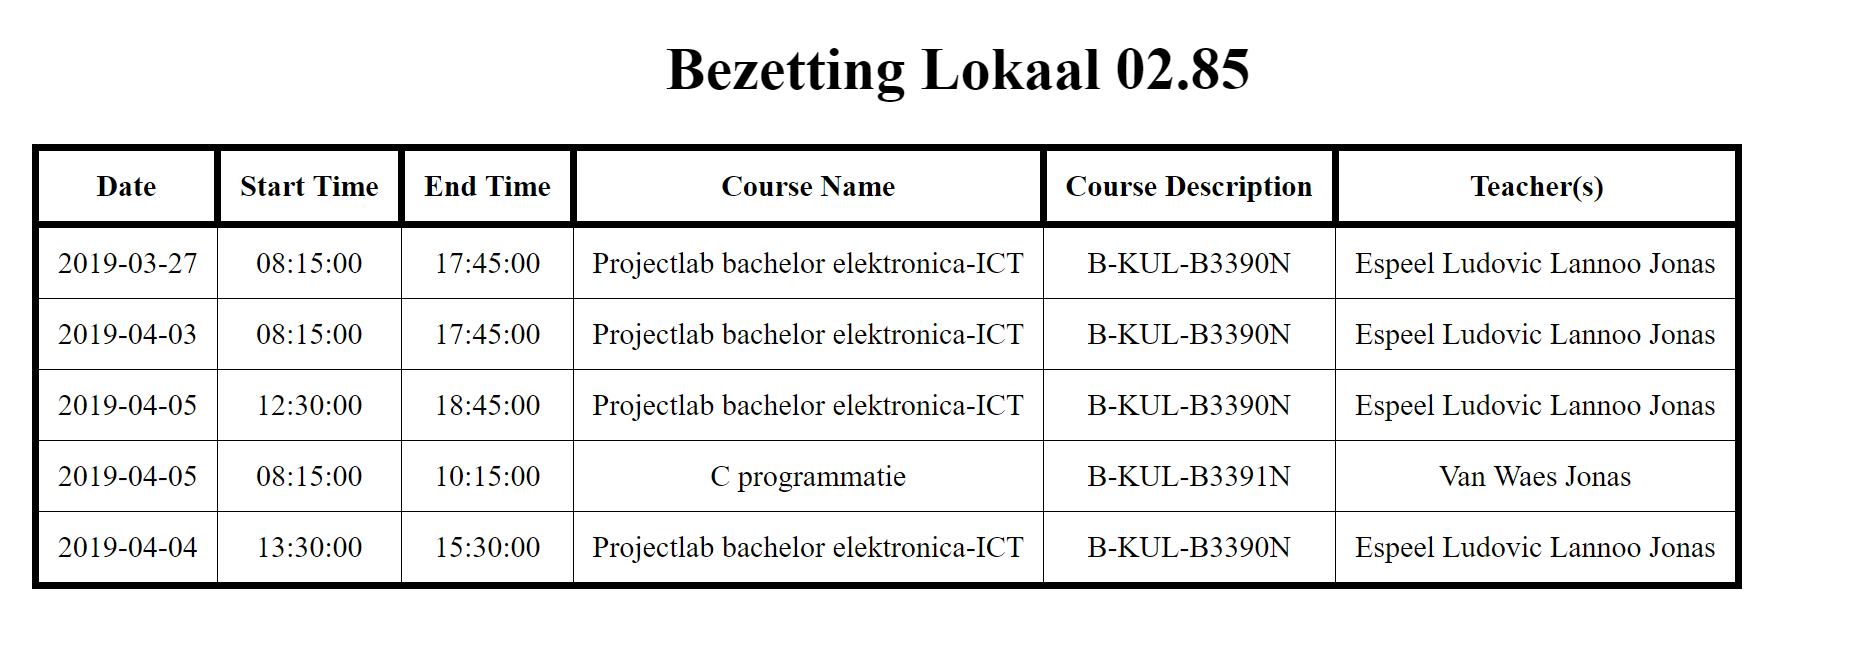
\includegraphics[width=1\textwidth]{vbDatabank}
	\caption{lokaalbezetting lokaal 02.85}
	\label{fig:vboutput}
\end{figure}

Wanneer we merkten dat dit werkte, hebben we daar nog data aan toegevoegd. Ook slaan we de data niet meer op in een bestand, omdat we dit moeilijk kunnen doorsturen. Nu kunnen we de info van lokaal 02.85 filteren op 4 april 2019. Zie figuur \ref{fig:vbdata}. Alles staat nu als tekst na elkaar. Dit is gemakkelijker om door te sturen. Eens het doorgestuurd is, kunnen we er opnieuw de juiste data uit filteren en er een tabel van maken om op een overzichtelijke manier op de display weer te geven.

\begin{figure}[h]
	\centering
	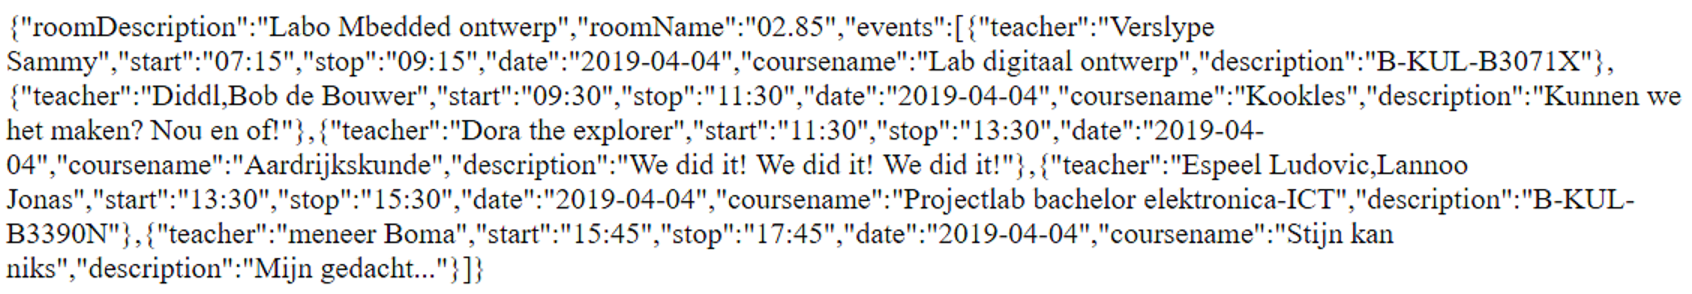
\includegraphics[width=1\textwidth]{vbData02_85}
	\caption{lokaalbezetting lokaal 02.85 op 04/04/2019}
	\label{fig:vbdata}
\end{figure}

We kunnen ook een figuur op de E-ink display afbeelden. Figuur \ref{fig:vbscherm} is een voorbeeld van voor we de data uit de databank konden doorsturen. Hier staan dus nog geen lessen in, maar het toont de lay-out van de display.
\newline
\begin{figure}[h]
	\centering
	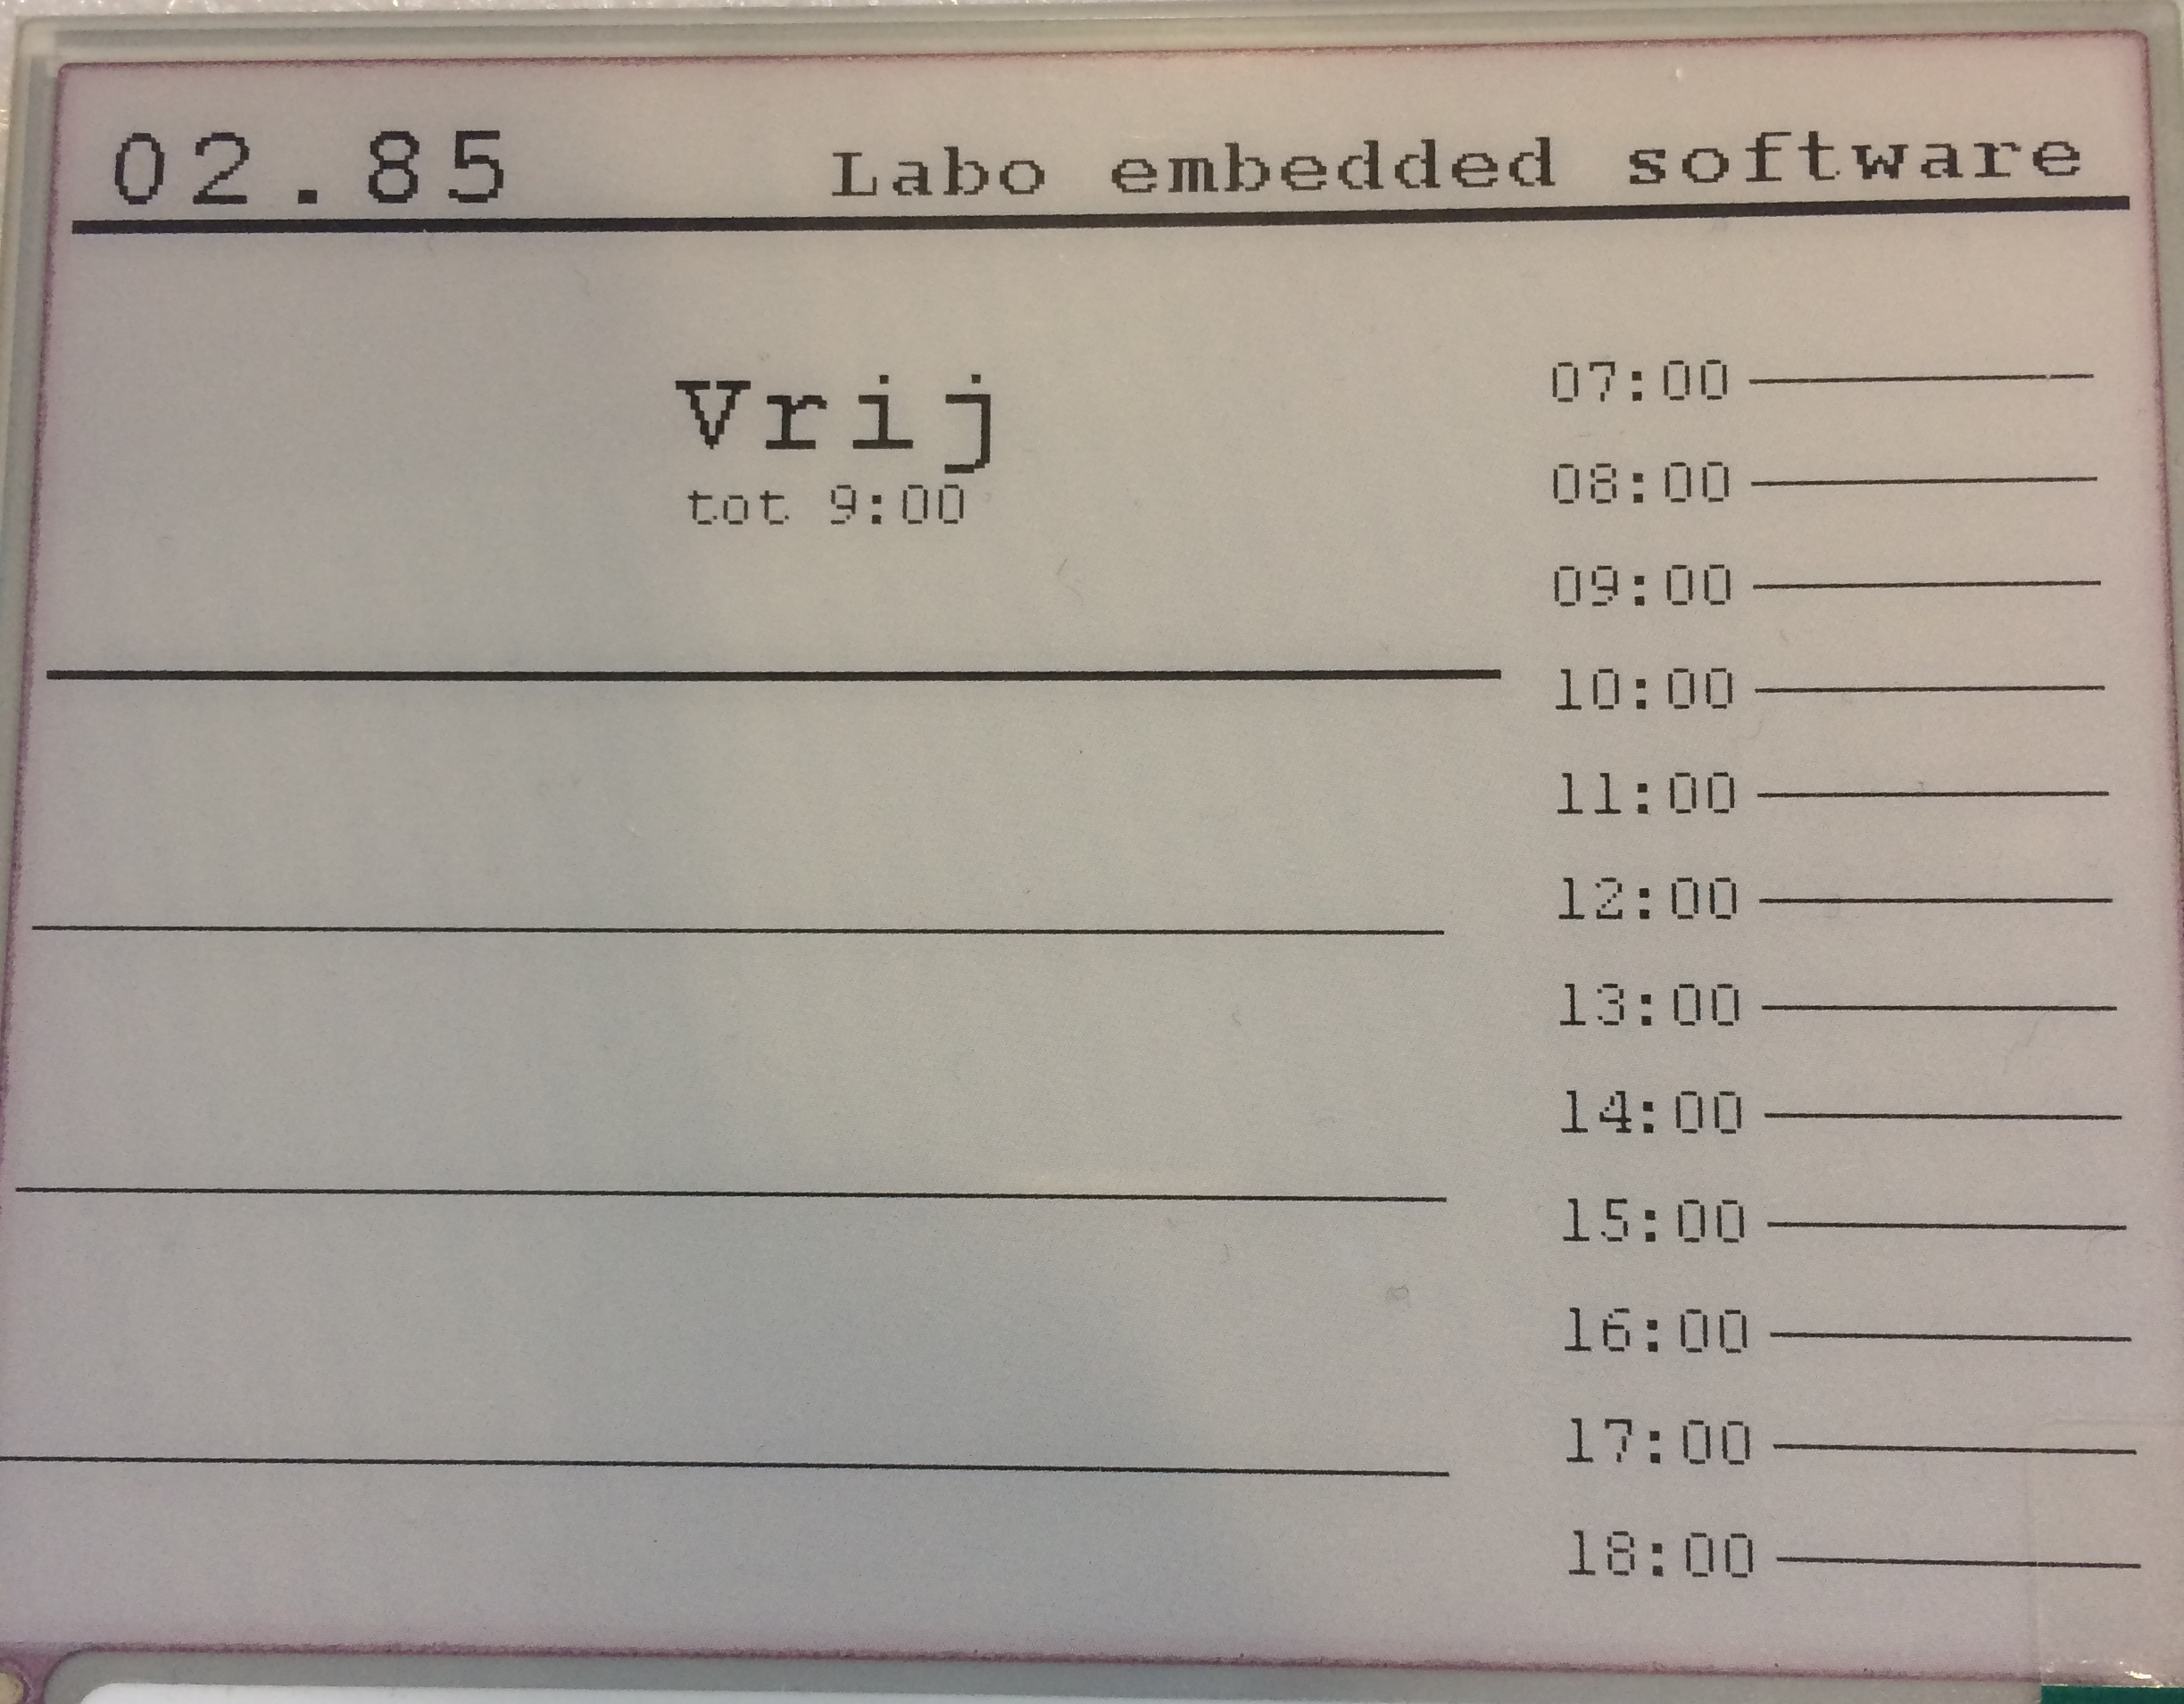
\includegraphics[width=0.75\textwidth]{vbScherm}
	\caption{E-ink display}
	\label{fig:vbscherm}
\end{figure}

De database en het accesspoint waren relatief snel opgezet. Ook iets afbeelden op de display ging relatief vlot. Het moeilijkste was om de data te kunnen versturen naar de display. Het was ook niet eenvoudig om een framebuffer te maken, omdat we dachten dat het niet mogelijk was om een buffer te maken van het hele scherm. We hebben het scherm dus moeten verdelen zodat we voor elk stuk apart een buffer konden maken en zo het scherm stuk per stuk up te daten.

\newpage

\section{In het vervolg}

Als we dit project verder zouden uitwerken, zouden we een andere mbed en wifi module gebruiken. Nu hebben we veel tijd verloren met het zoeken naar hoe we iets moeten implementeren. We zouden kunnen werken met modules die we kennen, waardoor alles sneller zou kunnen gaan. 
\newline
\newline
We hebben veel tijd verloren door te zoeken naar hoe we een framebuffer van heel het scherm kunnen maken. We dachten dat dat niet mogelijk was, dus hebben we een oplossing gezocht om een buffer van een deel van het scherm te maken. Dit was niet gemakkelijk en heeft veel tijd ingenomen. Achteraf hebben we gehoord dat het wel mogelijk is om heel het scherm in één keer up te daten. We zouden dus kunnen uitzoeken hoe dat werkt en het scherm op die manier implementeren, omdat het updaten van het scherm zo sneller zou gaan. 
\newline
\newline
Verder zouden we ook tijdens het zoeken naar oplossingen proberen meer geduld te hebben. Als er problemen waren met dingen die we niet begrepen, zouden we moeten efficiënter zoeken naar oplossingen. We zouden kunnen één manier van werken proberen volledig uit te werken en te begrijpen, in plaats van telkens iets kleins niet lukt, een volledig nieuwe manier te zoeken.

\newpage

\section{Conclusie}

We hebben een manier gevonden om op een energie zuinige manier een leslokaal dynamisch aan te duiden. We kunnen op een E-ink display aanduiden op welke uren van de dag het lokaal vrij is. Wanneer het lokaal niet vrij is, is duidelijk wie in het lokaal zit, welk vak er op dat moment gegeven wordt en hoe lang het nog zal duren voor het lokaal  weer vrij is.

\newpage

\bibliographystyle{plain}
\bibliography{library}

\end{document}
